\documentclass[12pt, twoside]{article}
\usepackage[letterpaper, margin=1in, headsep=0.2in]{geometry}
\setlength{\headheight}{0.6in}
%\usepackage[english]{babel}
\usepackage[utf8]{inputenc}
\usepackage{microtype}
\usepackage{amsmath}
\usepackage{amssymb}
%\usepackage{amsfonts}
\usepackage{siunitx} %units in math. eg 20\milli\meter
\usepackage{yhmath} % for arcs, overparenth command
\usepackage{tikz} %graphics
\usetikzlibrary{quotes, angles}
\usepackage{graphicx} %consider setting \graphicspath{{images/}}
\usepackage{parskip} %no paragraph indent
\usepackage{enumitem}
\usepackage{multicol}
\usepackage{venndiagram}

\usepackage{fancyhdr}
\pagestyle{fancy}
\fancyhf{}
\renewcommand{\headrulewidth}{0pt} % disable the underline of the header
\raggedbottom
\hfuzz=2mm %suppresses overfull box warnings

\usepackage{hyperref}

\fancyhead[LE]{\thepage}
\fancyhead[RO]{\thepage \\ Name: \hspace{4cm} \,\\}
\fancyhead[LO]{BECA / Dr. Huson / Geometry\\*  Unit 13: Quadrilaterals \\* 30 March 2023}

\begin{document}

\subsubsection*{11.3 Homework: Mixed angle review }
\begin{enumerate}
  \item Given two parallel lines and a transversal, as shown. Apply the theorem, ``If a transversal intersects two parallel lines, then corresponding angles are congruent."
  \begin{center}
  \begin{tikzpicture}
    \draw [<->, thick] (1,2)--(9,2);
    \draw [<->, thick] (0,0)--(8,0);
    \draw [<->, thick] (4,-1)--(5.5,3);
    \node at (4.5,0.3) [left]{$5$};
    \node at (4.5,0.3) [right]{$6$};
    \node at (4.3,-0.3) [left]{$7$};
    \node at (4.3,-0.3) [right]{$8$};
    \node at (5.2,2) [above left]{$1$};
    \node at (5.2,2) [above right]{$2$};
    \node at (5,2) [below left]{$3$};
    \node at (5,2) [below right]{$4$};
  \end{tikzpicture}
  \end{center}
  \begin{enumerate}
    \item State the angle corresponding with $\angle 2$. \vspace{1cm}
    \item Given $m\angle 8 = 115^\circ$ and $m\angle 4 = 5x^\circ$. Find $x$. \vspace{2cm}
    \item Given $m\angle 7 = 65^\circ$. Find $m\angle 2$. \vspace{2cm}
    \item In a proof, what reason would justify $\angle 4 \cong \angle 5$? \rule{6cm}{0.15mm}
  \end{enumerate}

  \item Given two vertical angles, $m \angle 1 = 5x+9$, $m \angle 2 = 6x-1$. Find $m \angle 1$.\\
  For full credit, check by comparing to $m\angle 2$.
      \begin{flushright}
      \begin{tikzpicture}[scale=.7]
        \draw [<->, thick] (0,-1.5)--(10,1.5);
        \draw [<->, thick] (2,3.5)--(7,-3.5);
        \node at (3,.4){1};
        \node at (6,-.6){2};
      \end{tikzpicture}
      \end{flushright}

\newpage

    \item Express the result to the nearest thousandth.  \vspace{1cm}

      \begin{multicols}{2}
        \begin{enumerate}
          \item $\sin 35^\circ = $ \vspace{1cm}
          \item $\tan 70^\circ =$
          \item $\sin 78^\circ = $ \vspace{1cm}
          \item $\cos 12^\circ =$

        \end{enumerate}
      \end{multicols} \vspace{1cm}

  \item Given $m\angle R=48$ and $m\angle UST=110$. Find $m\angle U$.\\[1cm]
    \begin{tikzpicture}
      %\draw [->, thick] (0,0)--(5,5);
      \draw [<-, thick] (8,0)--(0,0)--(3,3)--(4.5,0);
      \draw [fill] (0,0) circle [radius=0.05] node[below]{$R$};
      \draw [fill] (4.5,0) circle [radius=0.05] node[below]{$S$};
      \draw [fill] (3,3) circle [radius=0.05] node[right]{$U$};
      \draw [fill] (7,0) circle [radius=0.05] node[below]{$T$};
    \end{tikzpicture}
    \vspace{2cm}


  \item On the graph below, draw $\overline{AB}$, with $A(5,3)$ and $B(-1,-3)$, labeling the end points. Determine and state the coordinates of the midpoint $M$ of $\overline{AB}$ and mark and label it on the graph.\\
    \begin{tikzpicture}[scale=.635]
      \draw [help lines] (-3,-2) grid (8,7);
      \draw [thick, ->] (-3.2,0) -- (8.4,0) node [below right] {$x$};
      \draw [thick, ->] (0,-2.2)--(0,7.4) node [left] {$y$};
    \end{tikzpicture}
    \vspace{1cm}

  \item In a proof, each of the following statements are written. Write down the reason that would justify each step. \bigskip
    \begin{enumerate}
      \item $\overline{PQ} \cong \overline{PQ}$ \hspace{4cm} $\rule{5cm}{0.15mm}$ property \bigskip
      \item $PQ+RS= QR+RS$  \hspace{1.7cm} $\rule{5cm}{0.15mm}$ property  \bigskip
      \item $2(PQ + QR)=2PQ+2QR$  \hspace{0.6cm} $\rule{5cm}{0.15mm}$ property
    \end{enumerate}

  \item Given right $\triangle JKL$ with $\overline{JK} \perp \overline{KL}$, $JL=8$, $m\angle J=30^\circ$.
    \begin{center}
      \begin{tikzpicture}[scale=0.7]
        \draw [thick](0,0)--(7,0)--(7,3)--(0,0);
        \draw [fill] (0,0) circle [radius=0.05] node[below]{$J$};
        \draw [fill] (7,0) circle [radius=0.05] node[below]{$K$};
        \draw [fill] (7,3) circle [radius=0.05] node[above right]{$L$};
        %\draw [color=blue] (0,0) ++(0.75,0) arc [start angle=0, end angle=70, radius=0.75];
        %\draw [color=blue] (4,0) ++(-0.22, 0.73) arc [start angle=110, end angle=180, radius=0.75];
        %\draw [thick] (0.8,3.1)--(1.2,2.9); %tick mark
        %\draw [thick] (2.8,2.9)--(3.2,3.1); %tick mark
        %\node [right] at (3.25,2.5){$x+7$};
        %\node [left] at (0.75,2.5){$2x+1$};
      \end{tikzpicture} \vspace{1cm}
    \end{center}
    \begin{enumerate}
      \item Find the length $JK$\\[2cm]
      \item Find the length $KL$\\[2cm]
    \end{enumerate}

  \item Given a circle $O$ with radius $6$.
  \begin{enumerate}
    \item Find the circumference of $O$. \vspace{2cm}
    \item Find the area of $O$. \vspace{2cm}
  \end{enumerate}

\newpage
\subsubsection*{Circle the appropriate equation and state the justification}
Use the postulates and theorems you have learned. You may abbreviate them as follows: ``def. of bisector," ``$\perp$ rays meet at $90^\circ$," ``complementary $\angle$s add to 90," ``linear pairs add to 180," ``vertical $\angle$s are $\cong$," ``corresponding $\angle$s of parallel lines are $\cong$."


\item Given $m\angle R=m\angle U =65$, and $m\angle UST=130$. Find $m\angle RSU$.
\begin{tikzpicture}[scale=0.6]
  %\draw [->, thick] (0,0)--(5,5);
  \draw [<-, thick] (7,0)--(1,0)--(3,3)--(4.5,0);
  \draw [fill] (1,0) circle [radius=0.05] node[below]{$R$};
  \draw [fill] (4.5,0) circle [radius=0.05] node[below]{$S$};
  \draw [fill] (3,3) circle [radius=0.05] node[right]{$U$};
  \draw [fill] (6,0) circle [radius=0.05] node[below]{$T$};
\end{tikzpicture}\\[0.5cm]
$\angle UST \cong \angle RSU$ \hspace{0.5cm} $m\angle UST + m\angle RSU =  180$ \hspace{0.5cm} \rule{6cm}{0.15mm} \vspace{0.5cm}

\item Given $\overrightarrow{BA} \perp \overrightarrow{BC}$, $m \angle ABD = 2x-5$, and $m \angle DBC = x-10$.
  \begin{tikzpicture}[scale=0.7]
    \draw [<->, thick] (0,3)--(0,0)--(5,0);
    \draw [->, thick] (0,0)--(3.5, 2);
    \draw [-, thin] (0, 0.4)--(0.4, 0.4)--(0.4, 0);
    \draw [fill] (0,0) circle [radius=0.05] node[below]{$B$};
    \draw [fill] (0,2) circle [radius=0.05] node[left]{$A$};
    \draw [fill] (4,0) circle [radius=0.05] node[below]{$C$};
    \draw [fill] (2.625, 1.5) circle [radius=0.05] node[below]{$D$};
  \end{tikzpicture}\\[0.5cm]
  $\angle ABD \cong \angle DBC$ \hspace{0.5cm} $m\angle ABD + m\angle DBC =  90$ \hspace{0.5cm} \rule{6cm}{0.15mm}


\item $\angle RPS \cong \angle SPU$ \hspace{0.25cm} $m \angle RPS + m \angle SPU = 180^\circ$ \hspace{0.25cm} \rule{6cm}{0.15mm}  \vspace{0.25cm}
    \begin{tikzpicture}[scale=0.7]
      \draw [<->, thick] (-5,.5)--(3,-.3);
      \draw [->, thick] (0,0)--(-1.2,3);
      \draw [fill] (-1,2.5) circle [radius=0.05] node[left ]{$S$};
      \draw [fill] (0,0) circle [radius=0.05] node[below]{$P$};
      \draw [fill] (2,-0.2) circle [radius=0.05] node[above]{$U$};
      \draw [fill] (-4,0.4) circle [radius=0.05] node[above]{$R$};
    \end{tikzpicture}


  \item Given corresponding angles of a transversal and two parallel lines, $\angle A$, $\angle B$.\\[0.5cm]
  $\angle A \cong \angle B$ \hspace{1cm} $m \angle A + m \angle B=180^\circ$ \hspace{0.5cm} \rule{5cm}{0.15mm} \vspace{0.25cm}

\item Given $m \angle 1 = 4x+6$, $m \angle 2 = 6x-32$. Find $m \angle 1$.
    \begin{tikzpicture}[scale=.4]
      \draw [<->, thick] (0,-1.5)--(10,1.5);
      \draw [<->, thick] (2,3.5)--(7,-3.5);
      \node at (3,.4){1};
      \node at (6,-.6){2};
    \end{tikzpicture}\\[0.5cm]
    $\angle 1 \cong \angle 2$ \hspace{1cm} $m\angle 1 + m\angle 2 =  180$ \hspace{0.5cm} \rule{6cm}{0.15mm}

\newpage

  \item Given $\overline{ABC}$, $AC=18$, and the point $B$ partitions $\overline{AC}$ in a ratio of $2{:}7$.\\[0.5cm] Find ${AB}$. \\[1.5cm]
      \begin{tikzpicture}
        \draw [-, thick] (1,0)--(7,0);
        \draw [fill] (1,0) circle [radius=0.05] node[below]{$A$};
        \draw [fill] (3.5,0) circle [radius=0.05] node[below]{$B$};
        \draw [fill] (7,0) circle [radius=0.05] node[below]{$C$};
      \end{tikzpicture} \vspace{3cm}


  \item Given $\overrightarrow{BA} \perp \overrightarrow{BC}$, $m \angle ABD = 4x$, and $m \angle DBC = 2x-12$. Find $m \angle DBC$. \\[0.5cm]
  For full credit, show the check using both angle measures.
    \begin{flushleft}
    \begin{tikzpicture}[scale=1.3]
      \draw [<->, thick] (0,3)--(0,0)--(5,0);
      \draw [->, thick] (0,0)--(3.5, 2);
      \draw [-, thin] (0, 0.4)--(0.4, 0.4)--(0.4, 0);
      %\node at (3,.4){1};
      %\node at (6,-.6){2};
      \draw [fill] (0,0) circle [radius=0.05] node[below]{$B$};
      \draw [fill] (0,2) circle [radius=0.05] node[left]{$A$};
      \draw [fill] (4,0) circle [radius=0.05] node[below]{$C$};
      \draw [fill] (2.625, 1.5) circle [radius=0.05] node[below]{$D$};
    \end{tikzpicture}
    \end{flushleft}
    \vspace{3cm}

  \item Given $P(3,4)$ and $Q(7,1)$, find the length of $\overline{PQ}$.
      \vspace{6cm}

  \item Given the circle $C$ with circumference $6\pi$.
  \begin{enumerate}
    \item Write down the formula for the circumference of a circle and solve for the radius yielding a circumference of $6\pi$. \vspace{1cm}
    \item Find the area of the circle.
  \end{enumerate}
  \begin{tikzpicture}[scale=.635]
    \draw [help lines] (-4,-4) grid (4,4);
    %\draw [thick, ->] (-2.2,0) -- (10.4,0) node [below right] {$x$};
    %\draw [thick, ->] (0,-2.2)--(0,10.4) node [left] {$y$};
    \draw (0,0) circle [radius=3] node[below]{$C$};
    \draw [fill] (0,0) circle [radius=0.05];
  \end{tikzpicture}

  \item On the graph, draw polygon ABCDEF with vertices A(1, 1), B(1, 4), C(3, 4), D(3, 7), E(8, 7), and F(8, 1). Find the perimeter and the area of the polygon.\\[1cm]
  \begin{tikzpicture}[scale=.635]
    \draw [help lines] (-2,-2) grid (10,10);
    \draw [thick, ->] (-2.2,0) -- (10.4,0) node [below right] {$x$};
    \draw [thick, ->] (0,-2.2)--(0,10.4) node [left] {$y$};
  \end{tikzpicture}
\vspace{2cm}

  
\end{enumerate}
\end{document}
  